\documentclass{article}

\usepackage[dblblindworkshop]{neurips_2026}
\workshoptitle{Transitioning from Pre-Training to Post-Training}

\usepackage[utf8]{inputenc}
\usepackage[T1]{fontenc}
\usepackage{hyperref}
\usepackage{url}
\usepackage{booktabs}
\usepackage{amsmath}
\usepackage{amsfonts}
\usepackage{microtype}
\usepackage{xcolor}
\usepackage{graphicx}

\makeatletter
\long\def\@makecaption#1#2{%
  \vskip\abovecaptionskip
  \sbox\@tempboxa{\footnotesize #1: #2}%
  \ifdim \wd\@tempboxa >\hsize
    {\footnotesize #1: #2\par}%
  \else
    \global \@minipagefalse
    \hb@xt@\hsize{\hfil\box\@tempboxa\hfil}%
  \fi
  \vskip\belowcaptionskip}
\makeatother

\title{What Changes During SVG Fine-Tuning?\
Separating Visual Discrimination from Executable Generation}

\author{Anonymous Author(s)}

\begin{document}
\nolinenumbers

\maketitle

\begin{abstract}
Post-training can make a model appear to acquire a new capability even when it mainly improves how existing knowledge is represented. We ask what supervised fine-tuning (SFT) changes in diagram-to-SVG reconstruction: the reliability of executable generation, the visual distinctions already available after pretraining, or both. We fine-tune pretrained Gemma~4 E4B on 1,995 image--SVG pairs from SVG-Diagrams and evaluate free generation at seven checkpoints against the unchanged base. A supporting diagnostic supplies valid original and edited SVGs and scores them by teacher-forced likelihood, so discrimination can be measured without requiring the model to generate code. On held-out source examples, executable validity rises from 3.1\% to 35.9\%, with no reliable final gain on either VFIG scientific-figure evaluation. The execution improvement is therefore specific to the training distribution. Validity and render-based fidelity reach half of their observed gain at the same checkpoint, so executable reconstruction improves early and together rather than as a syntax-first stage. SFT, therefore, chiefly improves executable SVG generation on the source distribution, while image-conditioned preference among valid candidates remains largely unchanged. Evaluations of structured-output post-training should distinguish successful program execution from information available to the model but not reliably expressed through generation.
\end{abstract}

\section{Introduction}

An improvement after supervised fine-tuning (SFT) does not, by itself, establish that post-training created a new capability. SFT may instead make pretrained knowledge easier to elicit, teach an output convention, or even improve the reliability of a long generation. Intermediate checkpoints therefore offer a direct way to examine this transition rather than comparing only the initial and final models \citep{biderman2023pythia,zhou2023lima}.

Diagram-to-SVG reconstruction makes these distinctions unusually visible. A model must recognize text, shapes, layout, and connectivity, and then express them as a long executable program. A prediction can preserve useful visual content yet fail because of malformed XML or incomplete termination; conversely, valid SVG can be structurally incorrect. Therefore, metrics computed after rendering mix visual reconstruction with successful code generation.

We follow a pretrained multimodal base model through one broad SVG SFT run. We focus on a single broad-SFT transition and leave structure-targeted data and curriculum comparisons to future work. We evaluate free generation at seven training checkpoints and compare it with the pretrained base. The main experiment asks whether improvements in executable SVG coincide with improvements in visual fidelity and whether they transfer beyond the source distribution. A smaller counterfactual diagnostic then supplies valid candidate SVGs and tests whether the model's preference changes with controlled edits to the image.

The study tests three expectations. First, if SFT primarily teaches the output format, executable validity should improve earlier than render-based fidelity. Second, if long serialization remains a bottleneck, non-closure and output-limit failures should persist after training. Third, if the base model already contains relevant visual information, controlled discrimination may succeed even when free generation is invalid.

The results obtained show a selective transition. SFT substantially improves executable generation on held-out data drawn from the same source as training, but the improvement does not transfer reliably to the two VFIG subsets. Moreover, validity and render-based fidelity rise at the same observed checkpoint, contrary to a simple syntax-first account. The candidate diagnostic suggests that some image--text correspondence is already present in the base model, whereas sensitivity to the sampled spatial and connector edits remains weak.

\begin{figure}[t]
  \centering
  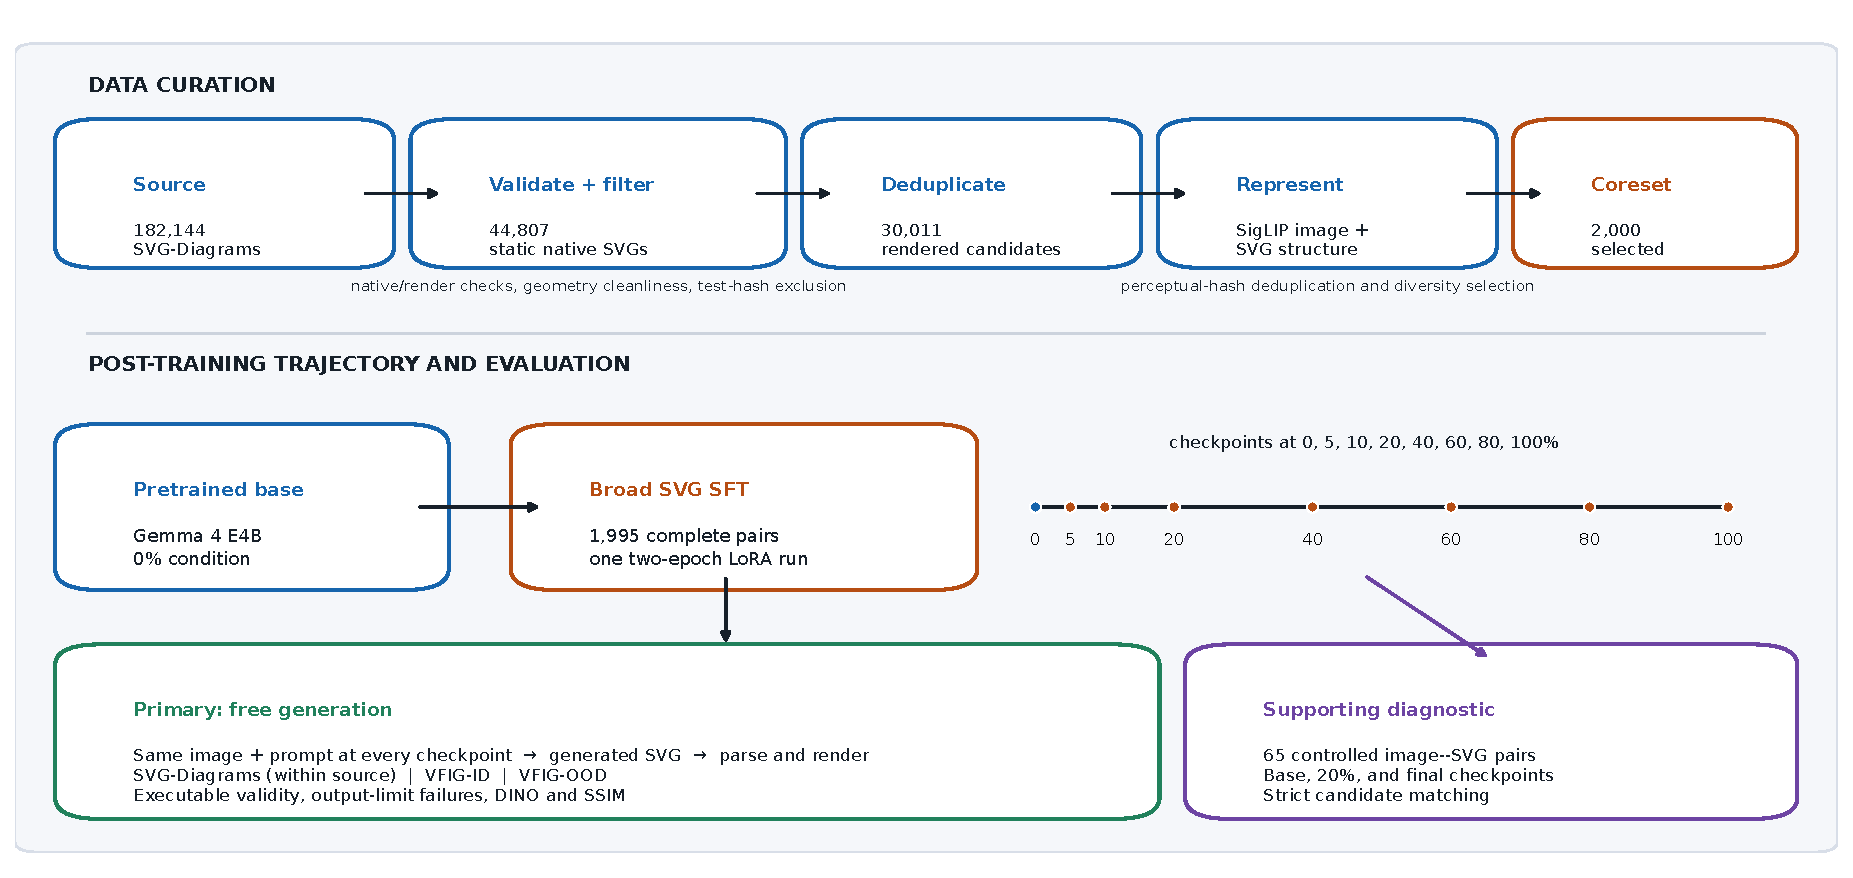
\includegraphics[width=\linewidth]{figures/experiment_overview.png}
  \caption{Curation of the SVG-Diagrams pool into 1,995 SFT pairs. Free generation is the primary evaluation; the candidate matching is a supporting diagnostic.}
  \label{fig:overview}
\end{figure}

\section{Related work}

StarVector introduced large-scale image-to-SVG modeling and the SVG-Diagrams corpus \citep{rodriguez2025starvector}, while VFIG extended this setting to complex scientific figures and emphasized errors in layout and connectivity that pixel metrics may miss \citep{he2026vfig}. Our focus is complementary: rather than optimizing final reconstruction quality, we measure behavioral change across a fixed SFT trajectory. The counterfactual diagnostic draws on likelihood-based visual scoring \citep{lin2024revisiting,ma2024examination} and paired contrastive evaluation \citep{gardner2020contrast,thrush2022winoground}, but applies them only to interpret failures of executable SVG generation.

\section{Study design}

\subsection{Training data and model trajectory}

We construct the training set from the SVG-Diagrams training split associated with StarVector. Figure~\ref{fig:overview} summarizes the curation process. Of 182,144 source examples, 44,807 satisfy the native-SVG validation and geometry-cleanliness criteria. Rendering and perceptual-hash deduplication reduce this pool to 30,011 candidates. We represent each candidate using a SigLIP image embedding together with structural SVG features, cluster the pool, and select 2,000 examples: 1,400 cluster medoids for broad coverage, 300 high-complexity cases, 200 examples from rare clusters, and 100 reserve selections. This procedure retains visual and structural variety under a fixed training budget rather than reproducing the source frequency distribution. The selected set contains 1,296 labeled diagrams, 687 workflow-like diagrams, and 17 geometry-like diagrams. Normalized SVG hashes exclude overlap with the held-out SVG-Diagrams test set; the audit finds no overlap among the 442 valid test hashes.

The progression from the source pool to the filtered coreset is intended to preserve heterogeneity while enforcing validity, deduplication, and a fixed training budget. This study therefore isolates the effect of ordinary broad SFT. It does not test whether structure-targeted data would change spatial or connector discrimination.

We fine-tune the pretrained, non-instruction-tuned Gemma~4 E4B model \citep{gemmateam2026gemma4} using LoRA \citep{hu2022lora}. Five selected examples do not fit as complete image--prompt--SVG sequences and are removed, leaving 1,995 training pairs. Cross-entropy is applied only to the target SVG tokens. We retain checkpoints at 5, 10, 20, 40, 60, 80, and 100\% of training and compare each with the unchanged pretrained base. Hyperparameters and serialization details are reported in Appendix~\ref{app:implementation}.

\subsection{Evaluation}

Free generation is evaluated on fixed, seeded subsets of 128 examples from each of three benchmarks. SVG-Diagrams supplies held-out examples from the training source and therefore measures within-source generalization. VFIG-Bench (VFIG-ID) contains more complex scientific diagrams with reference SVG, while VFIG-Bench-OOD contains curated scientific figures without reference SVG \citep{he2026vfig}. Every checkpoint receives the same image and reconstruction prompt and is decoded under the same output budget.

Our primary execution metric requires a prediction to parse as XML, satisfy a static native-SVG profile, contain drawable content, and render successfully. For benchmarks with references, we additionally report SSIM \citep{wang2004ssim} and DINO similarity \citep{caron2021dino}. Invalid generations receive zero similarity in the end-to-end analysis. This convention reflects practical utility, but it also makes fidelity depend on validity; the two curves cannot by themselves identify whether visual understanding or serialization changed first. Confidence intervals use paired resampling over examples.

To examine this coupling, we use a supporting diagnostic built from 65 source diagrams. Each example pairs an original SVG with a valid edited SVG and renders the corresponding images. Edits exchange text, box positions, connector endpoints, or text and box positions together. The model scores both SVG candidates under both images using length-normalized teacher-forced likelihood. Strict matching requires each image to prefer its corresponding SVG, thereby overcoming any fixed preference for one candidate. The probe is evaluated only at the base, 20\%, and final checkpoints. It measures discrimination among supplied alternatives, not the ability to construct an SVG freely; its construction and controls are detailed in Appendix~\ref{app:probe}.

\begin{figure}[t]
  \centering
  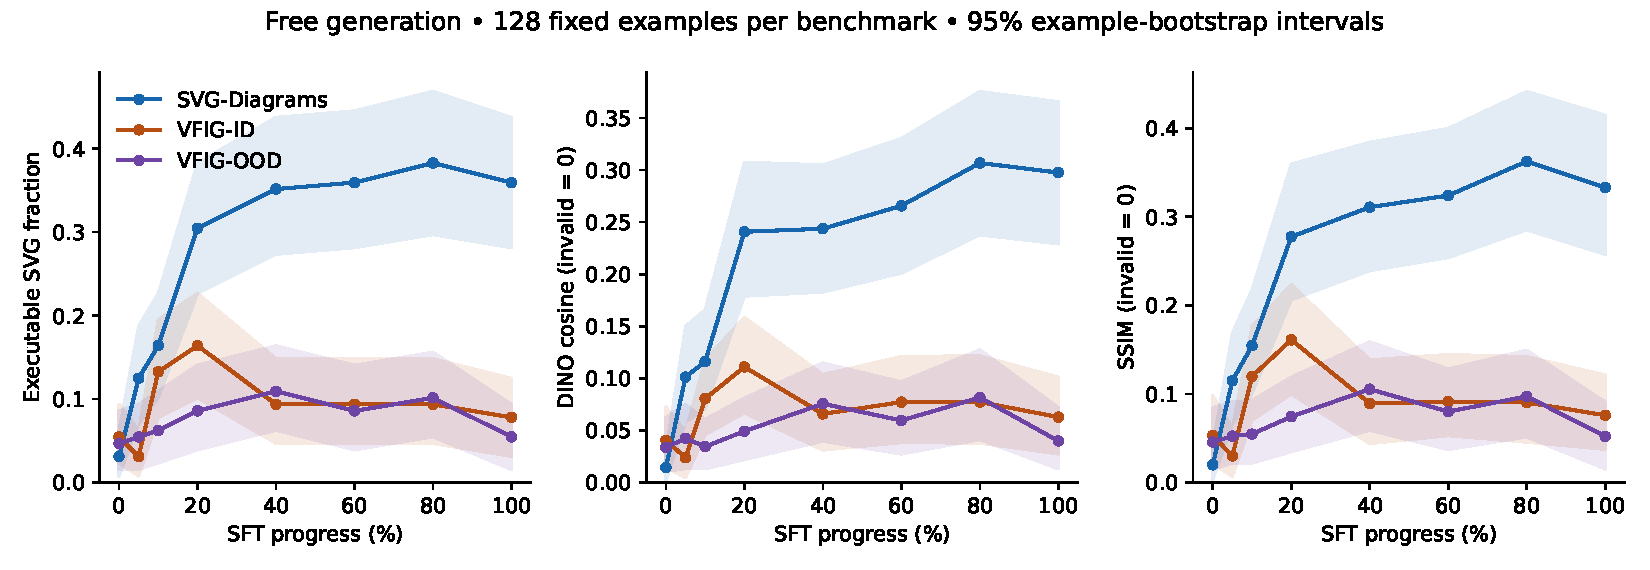
\includegraphics[width=\linewidth]{figures/svg_probe_generation_curves.pdf}
  \caption{Free generation across the pretrained base and its seven SFT checkpoints. Bands denote 95\% intervals over the same 128 examples at every checkpoint. DINO and SSIM assign zero to invalid outputs and therefore measure end-to-end reconstruction rather than visual fidelity in isolation.}
  \label{fig:generation}
\end{figure}

\section{Results}

\subsection{SFT improves execution within the source distribution}

Figure~\ref{fig:generation} shows a clear within-source improvement. On SVG-Diagrams, executable validity rises from 3.1\% at the base model to 12.5\% after only 5\% of SFT and to 30.5\% at the 20\% checkpoint. It peaks at 38.3\% at 80\% of training and ends at 35.9\%. The paired base-to-final change is 32.8 percentage points, with a 95\% interval of [24.2, 41.4]. DINO similarity rises from .014 to .298 and follows a similar trajectory. Validity, DINO, and SSIM all reach half of their base-to-final gain at the 20\% checkpoint. The dense checkpoint curve therefore shows early learning, but not earlier learning of validity relative to fidelity. This result does not support the preregistered syntax-first hypothesis. Moreover, because invalid predictions receive zero similarity, part of the joint movement is mechanical rather than independent evidence that visual reconstruction improves at the same rate.

The VFIG results are qualitatively different. Final validity changes from 5.5\% to 7.8\% on VFIG-ID and from 4.7\% to 5.5\% on VFIG-OOD. The paired changes are only 2.3 and 0.8 percentage points, and both confidence intervals include zero. Although validity reaches 16.4\% on VFIG-ID at the 20\% checkpoint and 10.9\% on VFIG-OOD at 40\%, these gains recede later in training. The non-monotonic curves caution against reporting only a favorable intermediate checkpoint as the outcome of SFT.

Termination and parsing account for much of the external failure. At the final checkpoint, 92.2\% of VFIG-ID and 94.5\% of VFIG-OOD generations exhaust the output budget, compared with 62.5\% on SVG-Diagrams. The final outputs include 118 XML parse failures on VFIG-ID and 121 on VFIG-OOD, out of 128 examples each. Only 13 VFIG-ID references exceed the 4,096-token generation budget, so reference length alone does not explain the failure rate. These results indicate that broad SFT improves executable generation on held-out examples from its source distribution without reliably transferring that behavior to more complex scientific figures.

\begin{table}[t]
  \caption{Base-to-final free generation on 128 held-out examples per benchmark. SVG-Diagrams is drawn from the training source; both VFIG subsets are external scientific figures. Invalid outputs receive DINO similarity zero.}
  \label{tab:generation}
  \centering
  \small
  \begin{tabular}{lccc}
    \toprule
    Benchmark & Executable validity & DINO similarity & Final output-limit rate \\
    \midrule
    SVG-Diagrams (held-out) & 3.1 $\rightarrow$ 35.9\% & .014 $\rightarrow$ .298 & 62.5\% \\
    VFIG-ID      & 5.5 $\rightarrow$ 7.8\%  & .041 $\rightarrow$ .063 & 92.2\% \\
    VFIG-OOD     & 4.7 $\rightarrow$ 5.5\%  & .034 $\rightarrow$ .040 & 94.5\% \\
    \bottomrule
  \end{tabular}
\end{table}

\subsection{Candidate matching changes little under SFT}

Strict matching on the 65 counterfactual pairs is essentially unchanged: 19 pairs succeed at the pretrained base and 20 at the final checkpoint. The aggregate likelihood interaction becomes more favorable to the correct image--SVG assignment, but this softer change rarely reverses both candidate rankings. Controls using unrelated images almost never satisfy the strict criterion, confirming that successful matches depend on the corresponding image rather than arbitrary image variation.

In percentage terms, strict matching changes from 29.2\% at the base model to 30.8\% after SFT, with substantially overlapping Wilson intervals. By contrast, the prior-canceling likelihood interaction $G$ increases from .0103 to .0142 nats per SVG token; the paired increase is .00385 with a 95\% interval of [.00187, .00658]. This distinction matters. Fine-tuning strengthens the average evidence favoring the correct joint image-SVG assignment, but the increase is usually too small to overcome the model's fixed preference for one SVG candidate on both images.

\begin{figure}[t]
  \centering
  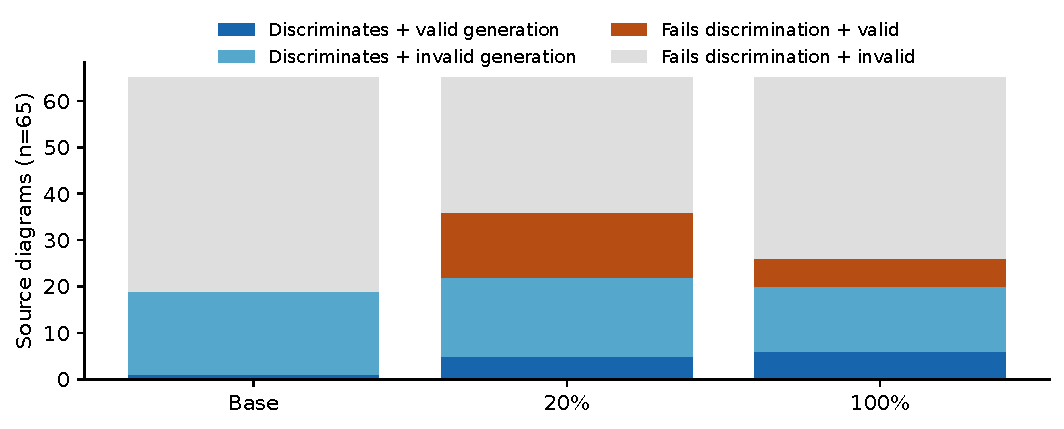
\includegraphics[width=0.82\linewidth]{figures/svg_probe_discrimination_generation.pdf}
  \caption{Relationship between strict candidate matching and executable free generation on the 65 diagnostic sources. Fine-tuning increases the number of valid generations, but many successfully matched sources still produce invalid SVG. The two evaluations therefore measure related but distinct behaviors.}
  \label{fig:discrimination-generation}
\end{figure}

The diagnostic also exposes a gap between recognition and generation (Figure~\ref{fig:discrimination-generation}). At the final checkpoint, only 6 of the 20 strictly matched sources also yield valid free generations; the remaining 14 match despite invalid generation. Conversely, 6 of the 12 sources with valid generations fail strict matching. On the balanced VFIG subset, text swaps are matched in 10/12 cases at the base and 11/12 at the final checkpoint, whereas box-position and connector-endpoint swaps produce 0/12 strict matches at every tested checkpoint. These strata are small and not matched for difficulty, so they locate a failure mode rather than establish a general hierarchy of visual skills. Detailed results and controls appear in Appendix~\ref{app:probe-results}.

\section{Discussion}

The observed transition is best described as an improvement in the expression of a structured-output capability, not evidence that SFT creates general diagram understanding. The roughly 33-point validity gain on SVG-Diagrams demonstrates that a small broad SFT set can sharply change executable behavior. Yet the absence of a reliable final gain on VFIG, together with the nearly unchanged strict matching rate, shows that this improvement is distribution-dependent. One plausible explanation is that SFT teaches common SVG serialization patterns and termination behavior represented in the source corpus. Another explanation is that it improves reconstruction only for diagrams similar to those examples. The present experiment cannot distinguish these mechanisms, and it does not show that post-training creates new visual representations.

The results also qualify the syntax-first hypothesis. Validity and end-to-end fidelity move together at the available checkpoints, both reaching $t_{50}$ at 20\% of SFT. Since invalid outputs are assigned zero fidelity, the current generation metrics cannot determine whether visual reconstruction improves independently of syntax. Scoring fidelity only among valid generations would introduce a different bias because the evaluated subset changes across checkpoints. The counterfactual diagnostic avoids both problems by supplying valid alternatives and reveals image-conditioned information behind some invalid outputs. It nevertheless measures recognition under teacher forcing and should not be interpreted as reconstruction performance.

Several limitations constrain the scope of the findings. We study one model, one SFT run, and one training-data source. The VFIG evaluation subsets are small relative to the full benchmarks, and the counterfactual edit strata contain few examples. As noted above, SVG-Diagrams and VFIG differ in diagram type, SVG length, and layout density, so the external null is a transfer result rather than a second draw from the same distribution. Because we do not compare broad supervision with a structure-targeted dataset, the results cannot determine whether a different data design would improve spatial or connector discrimination, or transfer to scientific figures. Finally, the training serialization and inference stopping conventions use different special tokens, so output-limit behavior may partly reflect protocol mismatch (Appendix~\ref{app:implementation}). Replication across seeds and model families, and a controlled termination ablation, are needed before treating these limits as properties of post-training in general.

\section{Conclusion}

Across one base-to-SFT trajectory, broad SVG supervision substantially improves executable generation within the data source but does not reliably transfer to complex scientific figures. A supporting candidate-matching diagnostic finds visual information in the pretrained base that often remains inaccessible through valid free generation, while sampled spatial and connector distinctions change little. Separating execution from visual discrimination yields a more precise account of what structured-output post-training changes.

\bibliographystyle{plainnat}
\bibliography{references}

\appendix
\section*{Appendix}
The appendix reports training and decoding details, the candidate-matching protocol, additional probe results by edit type, and a reproducibility and ethics note.

\section{Implementation and evaluation details}
\label{app:implementation}

Training uses rank-16 LoRA with scaling parameter 32, dropout 0.05, and adapters on all linear modules. The frozen base model and adapters use bfloat16. Raster inputs are letterboxed to $960\times960$. We train for two epochs with learning rate $10^{-4}$, effective batch size 8, and an 8,192-token context, for 500 optimizer steps. The seven saved adapters correspond to steps 25, 50, 100, 200, 300, 400, and 500. Complete examples that exceed the context are discarded rather than truncated.

Free generation uses greedy decoding with a 4,096-token output budget. We use 4,000 paired bootstrap resamples over examples for confidence intervals and an exact McNemar test for base-to-final changes in executable validity. The completed SFT run serialized assistant completions with the chat-template turn terminator, whereas generation used the tokenizer's declared end-of-sequence token. We therefore treat output-limit and termination results as potentially protocol-confounded pending a direct stopping-token ablation.

\section{Counterfactual diagnostic}
\label{app:probe}

For candidate SVG $c$ with $T$ tokens, image $x$, and fixed prompt $q$, the score is
\begin{equation}
  s_\theta(x,c)=\frac{1}{T}\sum_{t=1}^{T}\log p_\theta(c_t\mid x,q,c_{<t}).
\end{equation}
Within each pair, the original and edited SVG have identical token counts. For images $x_0,x_1$ and candidates $c_0,c_1$, we define
\begin{align}
  d_0 &= s_\theta(x_0,c_0)-s_\theta(x_0,c_1), \\
  d_1 &= s_\theta(x_1,c_1)-s_\theta(x_1,c_0).
\end{align}
Strict matching requires $d_0>10^{-6}$ and $d_1>10^{-6}$. The secondary interaction $G=d_0+d_1$ cancels any additive candidate-only preference but does not require both rankings to be correct. White images quantify candidate priors, and unrelated images test whether arbitrary image changes induce reversals. Pair construction was completed before the main diagnostic scores were produced, and no example was excluded on the basis of model performance.

The final set contains 24 text, 12 box-position, 13 connector-endpoint, and 16 combined edits. All candidates parse and render and were visually inspected. Two candidates fail the stricter executable-generation profile; excluding them does not change the qualitative comparison. The constructibility filter means that the probe applies only to diagrams admitting visible, equal-token edits of these forms.

\section{Additional counterfactual results}
\label{app:probe-results}

\begin{figure}[h]
  \centering
  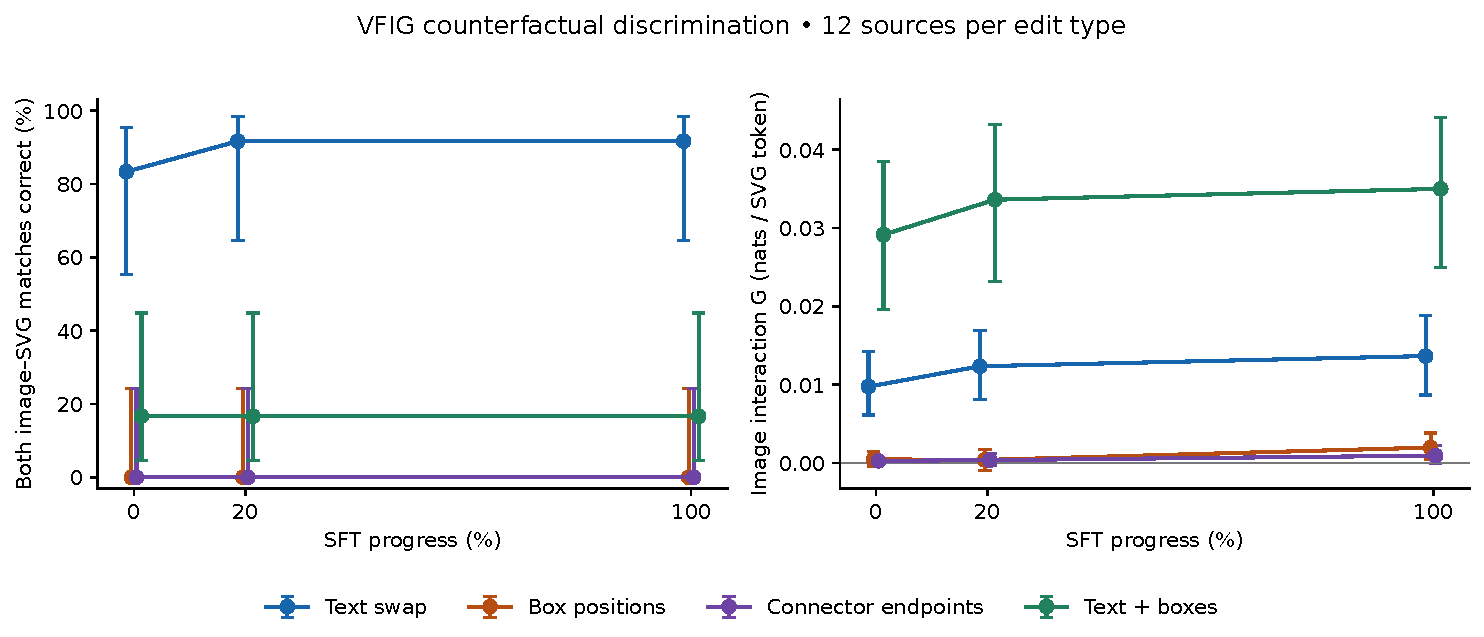
\includegraphics[width=\linewidth]{figures/svg_probe_by_edit.pdf}
  \caption{Counterfactual results on the balanced VFIG-ID subset ($n=12$ per edit type). Strict matching requires both image--candidate rankings to be correct. The interaction $G$ tests the preferred joint assignment after canceling fixed candidate preferences. Intervals are Wilson intervals for rates and example-bootstrap intervals for $G$.}
  \label{fig:probe}
\end{figure}

At the base, 20\%, and final checkpoints, strict matching succeeds on 19/65, 22/65, and 20/65 examples, respectively. At the final checkpoint, unrelated images succeed on 2/65 examples, while white images favor the original candidate in 62/65 pairs. The final-minus-base change in strict matching is one example; the paired change in $G$ is positive, indicating a stronger but generally insufficient image-dependent preference. On the balanced VFIG subset, final strict matching succeeds on 11/12 text edits, 0/12 box edits, 0/12 connector edits, and 2/12 combined edits. The Wilson upper bound for either 0/12 result is 24.2\%, underscoring the limited precision of these strata.

\begin{figure}[h]
  \centering
  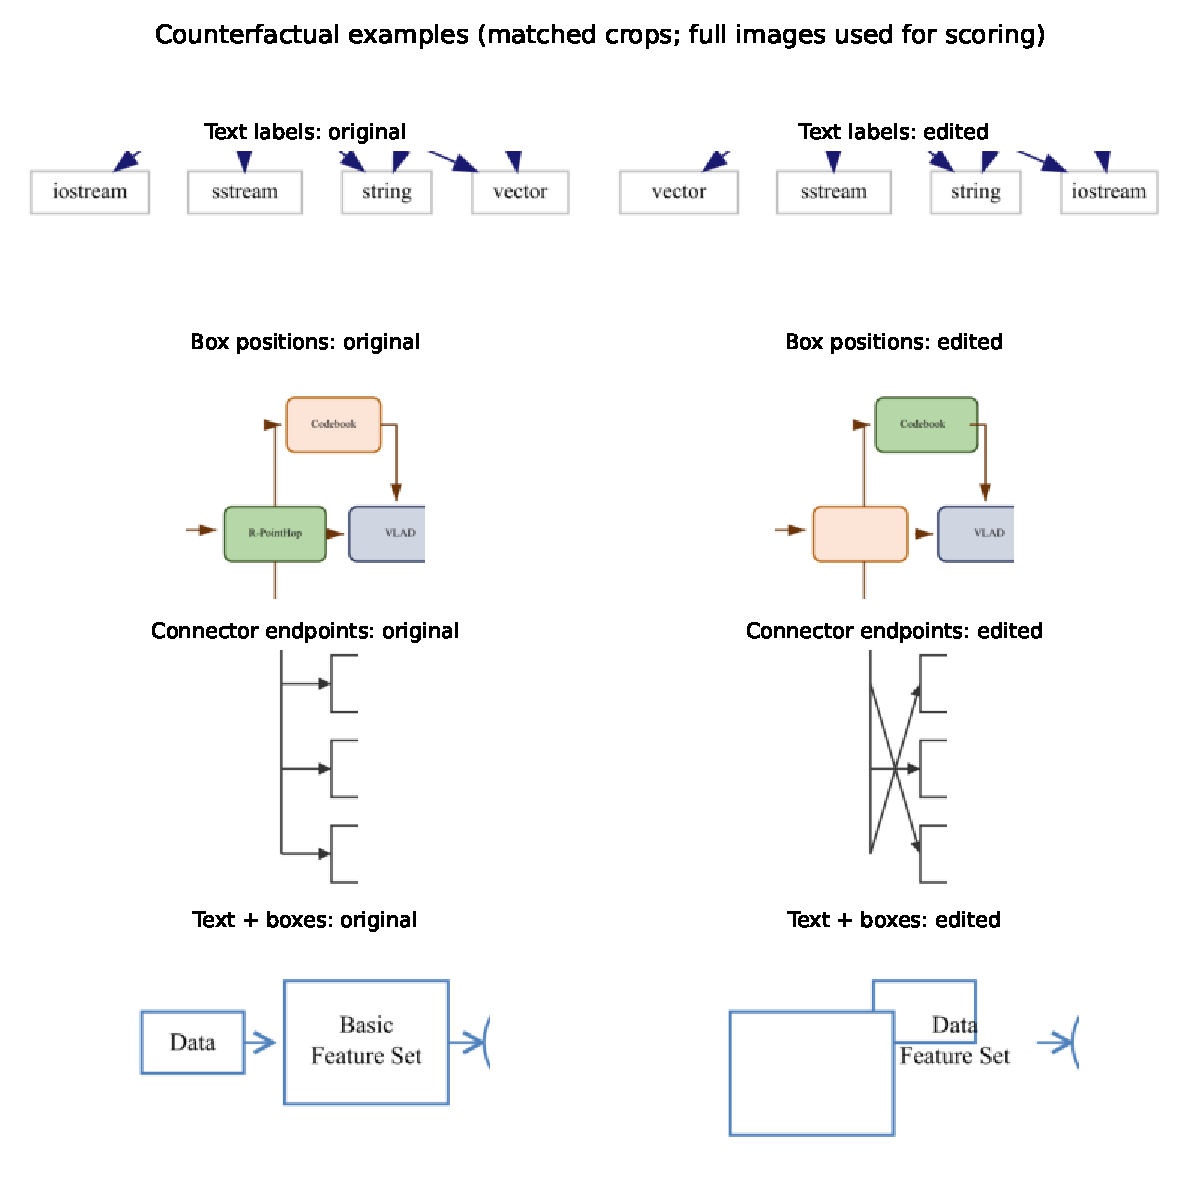
\includegraphics[width=0.9\linewidth]{figures/svg_probe_examples.pdf}
  \caption{Outcome-independent examples selected during the pre-score visual audit. Crops show the edited region; scoring uses the full $960\times960$ images.}
  \label{fig:examples}
\end{figure}

\section{Reproducibility and ethics}

The repository retains the training configuration, frozen evaluation subsets, cached generations, counterfactual candidates, raw likelihood scores, and scripts used to reproduce the reported analyses and figures. Processed data and model artifacts will be distributed subject to the licenses of the source datasets and model. The study uses public diagram datasets and pretrained model artifacts and involves no human participants or personal data. Parameter-efficient fine-tuning and a single main training run limit compute use.

\end{document}
